\section{Serotonin and Values}

\begin{quotex}
Your time is precious \& fleeting …Spend time with those who light ? up your life and enrich your existence. Make each moment count. \flright{\textsc{Anthony Hopkins}}

One Law for the Lion \& Ox is Oppression. \flright{\textsc{William Blake}, \emph{The Marriage of Heaven and Hell}}

To be popular, it is advisable to give people what they want, not what they need. Usually, that involves sentimentalism. Frithjof Schuon tells this story about Abd al-Qadir al-Jilani:

The saint relates a story about cats and the whole audience begins to weep from spiritual emotion.

They listened with boredom to the brilliant sermon of the great theologian. 

\end{quotex}
The most important factor in the soul of the human being is not race, nor ethnicity, nor intelligence, nor psychological type. It is one's real caste. Unfortunately, in a disordered age, this may not correspond to your imputed caste in your social milieu.

\begin{wrapfigure}{rt}{.3\textwidth}
 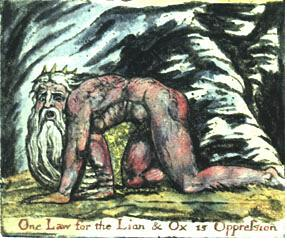
\includegraphics[scale=.5]{a20210912SerotoninandValues-img001.jpg}
\end{wrapfigure}

It governs one's understanding of knowledge, ethics, the good life, or friendship, among others. Because of the widespread usage of social media, the differences are readily apparent, much more so than in previous times because the voices of the lower castes are now so dominant. These are not value judgments, because it would be inappropriate, if not actually impossible, for the castes to be confused.

\paragraph{Two Misconceptions}
There are two typical types of common comments, which may sound intelligent superficially, but are not:

\begin{enumerate}
\item Broad negative generalizations that apply to everyone indiscriminately. 
\item ``what we need is XXX" type of argument 
\end{enumerate}
Of course, the author of these types of comments seldom realizes that he is part of that generalization or that he needs XXX also. We can simplify things and reduce them to two primal principles:

\begin{enumerate}
\item Humans are subject to the conditions of ignorance, concupiscence, maliciousness, and weakness. Anything else is a commentary on those four. 
\item Humans are ``rational animals", at least in potential, so what we ``need" is to actualize that power. In particular, rationality means the ability to choose the good, which in turn requires knowledge of the good. 
\end{enumerate}
Instead of the Hindu names, I'll refer to the four principal orientations as the spiritual, political, merchant, and servile types, without holding to rigid categories. The political type includes those who are attracted to administrative, legislative, judicial, and military careers. The merchant types run businesses or create things, and the servile type prefer manual labor.

As examples, I'll illustrate how the types approach certain categories. Taking these factors into consideration will reveal much about social life and its potential conflicts. Note that there is no question of one caste being superior to another. Quite the contrary, since a member of one is satisfied with his state and has no desire to imitate another.

\paragraph{The Good Life}
Those dominated by the conditions listed in (1) experience the good life as ``feeling good"

\paragraph{Knowledge}
\begin{itemize}
\item \textbf{Spiritual}: knowledge is metaphysics which leads to \emph{wisdom}. 
\item \textbf{Political}: knowledge is the application of metaphysical principles in the world, which develops \emph{power}. 
\item \textbf{Merchant}: knowledge is practical which leads to \emph{success}. 
\item \textbf{Servile}: knowledge is ``how-to" which leads to \emph{competence}. 
\end{itemize}
\paragraph{Distinctions of people}
\begin{itemize}
\item \textbf{Spiritual}: People are either those who know or those who believe. 
\item \textbf{Political}: They see the world in terms of friends and enemies. 
\item \textbf{Merchant}: For the merchant everyone is a potential customer. 
\item \textbf{Servile}: There are those who bring pleasure into their lives and those who do not. 
\end{itemize}
\paragraph{Reading Preferences}
These lists are not exhaustive.

\begin{itemize}
\item \textbf{Spiritual}: Metaphysics, literature, poetry, science. 
\item \textbf{Political}: History, political theory, military history. 
\item \textbf{Merchant}: Biographies, motivational, financial, prospectuses. 
\item \textbf{Servile}: Manuals, do-it-yourself videos. 
\end{itemize}
\paragraph{The Good Life}
We could continue with ethics, friendship, and more, much of which has already been covered elsewhere. The ultimate question, which determines the answers to the other categories, is what you consider to be the good life. Aristotle had his own hierarchy of needs predating Maslow: one desires:

\begin{enumerate}
\item To Live 
\item To Live Well 
\item To Live Better 
\end{enumerate}
Once you can survive, once you have achieved some consistency in your life, then what is your best life? Are you driven by the desire to think, to know, to understand, to serve the Good? Or do you prefer to ``feel good" by increasing your serotonin levels?

As an appendix, I'll include these thoughts by Anthony Hopkins, which many consider to be a guide for the good life. Does it help you to become wise? There is nothing about knowing, loving, or serving God.

\paragraph{I Need This in My Life}
Let go the people who are not prepared to love you. This is the hardest thing you will have to do in your life and it will also be the most important thing. Stop having hard conversations with people who don't want change.

Stop showing up for people who have no interest in your presence. I know your instinct is to do everything to earn the appreciation of those around you, but it's a boost that steals your time, energy, mental and physical health.

When you begin to fight for a life with joy, interest and commitment, not everyone will be ready to follow you in this place. This doesn't mean you need to change what you are, it means you should let go of the people who aren't ready to accompany you.

If you are excluded, insulted, forgotten or ignored by the people you give your time to, you don't do yourself a favor by continuing to offer your energy and your life. The truth is that you are not for everyone and not everyone is for you.

That's what makes it so special when you meet people who reciprocate love. You will know how precious you are.

The more time you spend trying to make yourself loved by someone who is unable to, the more time you waste depriving yourself of the possibility of this connection to someone else.

There are billions of people on this planet and many of them will meet with you at your level of interest and commitment.

The more you stay involved with people who use you as a pillow, a background option or a therapist for emotional healing, the longer you stay away from the community you want.

Maybe if you stop showing up, you won't be wanted. Maybe if you stop trying, the relationship will end. Maybe if you stop texting your phone will stay dark for weeks. That doesn't mean you ruined the relationship, it means the only thing holding it back was the energy that only you gave to keep it. This is not love, it's attachment. It's wanting to give a chance to those who don't deserve it. You deserve so much, there are people who should not be in your life.

The most valuable thing you have in your life is your time and energy, and both are limited. When you give your time and energy, it will define your existence.

When you realize this, you begin to understand why you are so anxious when you spend time with people, in activities, places or situations that don't suit you and shouldn't be around you, your energy is stolen.

You will begin to realize that the most important thing you can do for yourself and for everyone around you is to protect your energy more fiercely than anything else. Make your life a safe haven, in which only compatible people are allowed.

You are not responsible for saving anyone. You are not responsible for convincing them to improve. It's not your work to exist for people and give your life to them! If you feel bad, if you feel compelled, you will be the root of all your problems, fearing that they will not return the favours you have granted. It's your only obligation to realize that you are the love of your destiny and accept the love you deserve.

Decide that you deserve true friendship, commitment, true and complete love with healthy and prosperous people. Then wait and see how much everything begins to change. Don't waste time with people who are not worth it. Change will give you the love, the esteem, happiness and the protection you deserve.



\flrightit{Posted on 2021-09-12 by Cologero }

\begin{center}* * *\end{center}

\begin{footnotesize}\begin{sffamily}



\texttt{Greg on 2021-09-15 at 10:33 said: }

What does salvation and spirituality look like for the different casts. Since all casts have produced saints How does their sanctity differ?


\end{sffamily}\end{footnotesize}
